\documentclass{article}
% Change page layout
\usepackage[margin=2cm]{geometry}
\usepackage{xcolor}
\usepackage{parskip}
\usepackage{amsmath, amssymb}
\usepackage{hyperref}
\usepackage{graphicx}
\usepackage{caption}
\usepackage{svg}
\usepackage{placeins}
\usepackage{tikz}
\usetikzlibrary{positioning,3d}

\hypersetup{
    colorlinks=true
}

\let\vec\mathbf

\begin{document}
\input{../../assignmenttitle.tex}
\assignmenttitle{Classical Electrodynamics II}{Assignment 1}

\emph{Code link:} \url{https://github.com/Newtech66/TIFR-ED2} 

\section*{P1}
\subsection*{(i)}
\begin{figure}[h!]
  \begin{center}
    \includesvg[width=0.6\textwidth]{figs/0.100_E_B}
  \end{center}
  \captionsetup{width=0.8\textwidth}
  \caption{Field line projections for a particle moving with a constant velocity $v=0.1c\hat{x}$.}
\end{figure}

\subsection*{(ii)}
\begin{figure}[h!]
  \begin{center}
    \includesvg[width=0.6\textwidth]{figs/0.900_E_B}
  \end{center}
  \captionsetup{width=0.8\textwidth}
  \caption{Field line projections for a particle moving with a constant velocity $v=0.9c\hat{x}$.}
\end{figure}

\subsection*{(iii)}
\begin{figure}[h!]
  \begin{center}
    \includesvg[width=0.6\textwidth]{figs/0.999_E_B}
  \end{center}
  \captionsetup{width=0.8\textwidth}
  \caption{Field line projections for a particle moving with a constant velocity $v=0.999c\hat{x}$.}
\end{figure}

\section*{P2}
\subsection*{(A)}
\begin{figure}[h!]
  \begin{center}
    \includesvg[width=0.6\textwidth]{figs/0.100_t_1_E_B_a_0.300_perp.svg}
  \end{center}
  \captionsetup{width=0.6\textwidth}
  \caption{Radiated field line projections for a particle moving with initial velocity $v_0=0.1c\hat{x}$ and acceleration $a=0.3c\hat{z}$ at time $t=1$.}
\end{figure}
\begin{figure}[h!]
  \begin{center}
    \includesvg[width=0.6\textwidth]{figs/0.100_t_2_E_B_a_0.300_perp.svg}
  \end{center}
  \captionsetup{width=0.6\textwidth}
  \caption{Radiated field line projections for a particle moving with initial velocity $v_0=0.1c\hat{x}$ and acceleration $a=0.3c\hat{z}$ at time $t=2$.}
\end{figure}
\FloatBarrier
\subsection*{(B)}
\begin{figure}[h!]
  \begin{center}
    \includesvg[width=0.6\textwidth]{figs/0.100_t_1_E_B_a_0.900.svg}
  \end{center}
  \captionsetup{width=0.6\textwidth}
  \caption{Radiated field line projections for a particle moving with initial velocity $v_0=0.1c\hat{x}$ and acceleration $a=0.9c\hat{x}$ at time $t=1$.}
\end{figure}
\begin{figure}[h!]
  \begin{center}
    \includesvg[width=0.6\textwidth]{figs/0.100_t_2_E_B_a_0.900.svg}
  \end{center}
  \captionsetup{width=0.6\textwidth}
  \caption{Radiated field line projections for a particle moving with initial velocity $v_0=0.1c\hat{x}$ and acceleration $a=0.9c\hat{x}$ at time $t=2$.}
\end{figure}
\FloatBarrier
We assume that the particle starts accelerating at $t=0$. We only plot the field line projections for $v=0.1c$ because it would be redundant to plot the rest. For part (B), the equations for velocity are given in \href{https://physics.stackexchange.com/questions/417841/relativistic-equation-for-motion-in-a-constant-acceleration}{this Physics StackExchange question.} We can follow the same procedure for part (A) and end up with the equations
\begin{gather}
    v = c\sqrt{\frac{k^2+a^2t^2}{c^2+k^2+a^2t^2}}\\
    \dot{x} = k\sqrt{1-\frac{v^2}{c^2}}\\
    \dot{z} = \frac{at}{k}\dot{x}
\end{gather}
The position of the particle over time is computed by numerically integrating the velocity.

\section*{P3}
\subsection*{(A)}
In this case, the velocity is along the x-axis and the acceleration is along the z-axis. So this is a case of the acceleration being perpendicular to the velocity. The answer is given by equation (4.103) of Rybicki and Lightman.
\begin{equation}
    \frac{dP}{d\Omega} = \frac{q^2a^2}{4\pi c^3}\frac{1}{(1-\beta cos\theta)^4}\left[1-\frac{\sin^2\theta\cos^2\phi}{\gamma^2(1-\beta\cos\theta)^2}\right]
\end{equation}
\begin{figure}[h!]
  \begin{center}
    \includegraphics[width=0.6\textwidth]{figs/q2perp.png}
  \end{center}
  \captionsetup{width=0.65\textwidth}
  \caption{As $\beta$ increases, the radiation gets more sharply peaked in the direction of motion. The plots here are normalized by the maximum value. We show a cross section so that the side lobes are visible.}
\end{figure}

\subsection*{(B)}
In this case, the velocity is along the x-axis and the acceleration is along the x-axis. So this is a case of the acceleration being parallel to the velocity. The answer is given by equation (4.101) of Rybicki and Lightman.
\begin{equation}
    \frac{dP}{d\Omega} = \frac{q^2a^2}{4\pi c^3}\frac{\sin^2\theta}{(1-\beta\cos\theta)^6}
\end{equation}
\begin{figure}[h!]
  \begin{center}
    \includegraphics[width=0.6\textwidth]{figs/q2parallel.png}
  \end{center}
  \captionsetup{width=0.65\textwidth}
  \caption{As $\beta$ increases, the radiation gets more sharply peaked in the direction of motion. The plots here are normalized by the maximum value.}
\end{figure}

\section*{P4}
\subsection*{(A)}
A free charge experiences a force $\vec{F}=q\vec{E}_{\text{in}}$. The dipole moment of a free charge is given by $\vec{d}=q\vec{r}$. That means
\begin{equation}
    \ddot{\vec{d}}=\frac{q^2}{m}\vec{E}_{\text{in}}
\end{equation}
Unpolarised light can always be decomposed into a superposition of two linearly polarised beams with polarisations along perpendicular axes with any orientation in the plane perpendicular to the direction of propagation. What this means is that we can always decompose the unpolarised light into one beam with a polarisation in the plane containing both the charged particle and the observation point, and one with a polarisation perpendicular to it.

\begin{figure}[h]
    \centering
    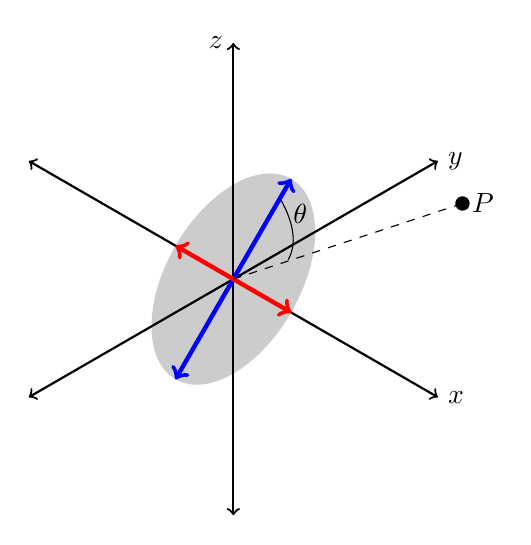
\begin{tikzpicture}[x={(0.866cm,-0.5cm)}, y={(0.866cm,0.5cm)}, z={(0cm,1cm)},scale=3]
\draw[<->, thick] (-1,0,0) -- (1,0,0) node[anchor=west] {$x$};
\draw[<->, thick] (0,-1,0) -- (0,1,0) node[anchor=west] {$y$};
\draw[<->, thick] (0,0,-1) -- (0,0,1) node[anchor=east] {$z$};
\begin{scope}[canvas is yz plane at x=0,scale=0.4]
\fill[opacity=0.2] (0,0) circle [radius=1];
\draw[<->, ultra thick,color=blue,rotate=45] (-1,0) -- (1,0);
\draw[<->, ultra thick,color=red,rotate=-45] (-1,0) -- (1,0);
\end{scope}
\draw[-, dashed, thin,scale=0.8] (0,0,0) -- (0.7, 0.7, 0.4);
\filldraw[scale=0.8] (0.7, 0.7, 0.4) circle [radius=1pt] node[anchor=west] {$P$};
\begin{scope}[x={(0.866cm,-0.5cm)}, y={(0.866cm,1.5cm)}]
\draw[-,scale=0.4] (0.4,0.27) arc[radius=0.2,start angle=0, end angle=36,x radius=2, y radius=0.5] node[above right=-0.2 and 0.24]{$\theta$};
\end{scope}
\end{tikzpicture}
    \caption{The incoming polarized light is split into two axes. The blue axis is in the plane containing the origin and the observation point $P$. The red axis is perpendicular to it. Note that the angle $\theta$ is measured in the plane containing the origin and $P$ and is not the $\theta$ in spherical coordinates. This is true of $\phi$ in part (C) as well.}
\end{figure}

The intensity of an oscillating dipole is given by equation (3.23a) of Rybicki and Lightman,
\begin{equation}
    \frac{dP}{d\Omega}=\frac{|\ddot{\vec{d}}|^2}{4\pi c^3}\sin^2\Theta
\end{equation}
where $\Theta$ is the angle between $\ddot{\vec{d}}$ and the vector to the observation point.

Consider the beam with polarisation in the plane. Let the angle between the in-plane polarisation vector and the position vector br $\theta$. So the intensity is
\begin{equation}
    \frac{dP_{\parallel}}{d\Omega}=\frac{q^2|\vec{E}|^2}{4\pi mc^3}\sin^2\theta
\end{equation}

Consider the beam with polarisation perpendicular to the plane. The out-of-plane polarisation vector and the position vector are perpendicular. So the intensity is
\begin{equation}
    \frac{dP_{\perp}}{d\Omega}=\frac{q^2|\vec{E}|^2}{4\pi mc^3}
\end{equation}
So the total intensity is
\begin{equation}
    \frac{dP}{d\Omega}=\frac{q^2|\vec{E}|^2}{4\pi mc^3}(1+\sin^2\theta)
\end{equation}
The degree of polarisation is
\begin{align}
    \Pi&=\frac{I_{\text{max}}-I_{\text{min}}}{I_{\text{max}}+I_{\text{min}}}\\
    &=\frac{1-\sin^2\theta}{1+\sin^2\theta}
\end{align}

\subsection*{(B)}
The intensity is invariant under $\theta\to\pi-\theta$. We get 100\% polarisation at $\theta=0$ and 0\% polarization at $\theta=\pi/2$.

\subsection*{(C)}
Let $\theta$ be the angle between the in-plane polarization vector of the beam propagating along $x$ and the position vector. Similarly let $\phi$ be the angle between the in-plane polarization vector of the beam propagating along $z$ and the position vector.  From the results of (A), we can get the total power as
\begin{equation}
    \frac{dP}{d\Omega}=\frac{q^2}{4\pi mc^3}|\vec{E}|^2(1+\sin^2\theta)+\frac{q^2}{4\pi mc^3}\frac{|\vec{E}|^2}{10}(1+\sin^2\phi)
\end{equation}
So the degree of polarisation is
\begin{equation}
    \Pi=\frac{(1-\sin^2\theta)+\frac{1}{10}(1-\sin^2\phi)}{(1+\sin^2\theta)+\frac{1}{10}(1+\sin^2\phi)}
\end{equation}

\section*{P5}
The radiation reaction force is given by
\begin{equation}
    F_{\text{rad}}  = \frac{2q^2\ddot{v}}{3c^3}
\end{equation}
We can find that
\begin{equation}
    \ddot{v}(t) = V_0\left(-900\cos(30t)+\frac{1}{10000}\sin(30t)\exp\left(\frac{t}{100}\right)+\frac{3}{5}\cos(30t)\exp\left(\frac{t}{100}\right)\right)
\end{equation}
\begin{figure}[h]
  \begin{center}
    \includegraphics[width=0.6\textwidth]{figs/q5.png}
  \end{center}
  \captionsetup{width=0.65\textwidth}
  \caption{The radiation reaction force oscillates very quickly, therefore it is plotted only up to 1 seconds, and not 1000 seconds as asked in the problem.}
\end{figure}

\section*{P6}
The emitted power density per unit frequency is given by Rybicki and Lightman equation (5.11).
\begin{equation}
    \frac{dW}{d\omega dVdt}(v,\omega)=\frac{16\pi e^6}{3\sqrt{3}c^3m^2 v}n_en_iZ^2g_{ff}(v,\omega)
\end{equation}
We need to do the integral
\begin{equation}
    \frac{dW}{d\omega dVdt}(T,\omega) = \frac{\int_{v_{\text{min}}}^\infty dv\ \frac{dW}{d\omega dVdt}(v,\omega)v^4\exp\left(-\frac{mv^2}{2kT}\right)\left(1+0.3\times\left(\frac{mv^2}{kT}\right)\right)}{\int_0^\infty dv\ v^4\exp\left(-\frac{mv^2}{2kT}\right)\left(1+0.3\times\left(\frac{mv^2}{kT}\right)\right)}
\end{equation}
where $v_{\text{min}}=\sqrt{2h\nu/m}$ and $\omega=2\pi\nu$.

First let us compute the denominator.
\begin{align}
    \int_0^\infty dv\ v^4\exp\left(-\frac{mv^2}{2kT}\right)\left(1+0.3\times\left(\frac{mv^2}{kT}\right)\right) &= \frac{1}{2}\left(\frac{2kT}{m}\right)^{5/2}\Gamma\left(\frac{5}{2}\right) + 0.3\times\left(\frac{2kT}{m}\right)^{5/2}\Gamma\left(\frac{7}{2}\right)\\
    &=0.94\sqrt{\pi}\left(\frac{2kT}{m}\right)^{5/2}
\end{align}
We straightforwardly used the properties and values of the gamma function in the above. Now we compute the numerator.
\begin{align}
    &=\frac{16\pi e^6}{3\sqrt{3}c^3m^2}n_en_iZ^2\int_{v_{\text{min}}}^\infty dv\ v^3\exp\left(-\frac{mv^2}{2kT}\right)\left(1+0.3\times\left(\frac{mv^2}{kT}\right)\right)g_{ff}(v,\omega)\label{eq:1}\\
    &=\frac{8\pi e^6}{3\sqrt{3}c^3m^2}n_en_iZ^2\bar{g}_{ff}(v,\omega)\left(\frac{2kT}{m}\right)^2\int_{h\nu/kT}^\infty dt\ t\exp\left(-t\right)\left(1+0.6t\right)\label{eq:2}\\
    &=\frac{8\pi e^6}{3\sqrt{3}c^3m^2}n_en_iZ^2\bar{g}_{ff}\left(\frac{2kT}{m}\right)^2\left[0.6\left(\frac{h\nu}{kT}\right)^2+2.2\left(\frac{h\nu}{kT}\right)+2.2\right]\exp\left(-\frac{h\nu}{kT}\right)
\end{align}
We extracted $g_{ff}$ as a thermal averaged constant in going from (\ref{eq:1}) to (\ref{eq:2}). So finally we get
\begin{equation}
    \frac{dW}{d\nu dVdt}(T,\omega) = \frac{3.28\pi e^6}{c^3m^2}n_en_iZ^2\bar{g}_{ff}\left(\frac{2kT}{\pi m}\right)^{-1/2}\left[0.6\left(\frac{h\nu}{kT}\right)^2+2.2\left(\frac{h\nu}{kT}\right)+2.2\right]\exp\left(-\frac{h\nu}{kT}\right)
\end{equation}
\begin{figure}[h]
  \begin{center}
    \includegraphics[width=0.6\textwidth]{figs/p6.png}
  \end{center}
  \captionsetup{width=0.65\textwidth}
  \caption{The emitted power density per unit frequency at (i) T=300 K and (ii) T=$10^6$ K.}
\end{figure}

\hrulefill
\end{document}